\documentclass[11pt,titlepage]{article}

\usepackage[french,american]{babel}
\usepackage[utf8]{inputenc}
\usepackage[T1]{fontenc}
\usepackage{lmodern}
\usepackage{amsmath,amsfonts,amssymb}
\usepackage{graphicx}
\usepackage[a4paper]{geometry}           % See geometry.pdf to learn the layout
%\geometry{landscape}                    % Activate for for rotated page 
                                         % geometry
%\usepackage[parfill]{parskip}           % Activate to begin paragraphs with an
                                         % empty line rather than an indent
\usepackage{graphicx}
\usepackage{amssymb}
\usepackage{epstopdf}
\usepackage{color}
\usepackage[tt]{titlepic}
\usepackage{fancyhdr}
\usepackage{secdot}
\usepackage{booktabs}
\usepackage{rotating}

% WD41, LRS/EPFL/PSI ----------------------------------------------------------
\usepackage{multirow}
\usepackage{tabularx}
\usepackage{ragged2e}                      % for '\RaggedRight' macro 
                                           % (allows hyphenation)
\newcolumntype{Y}{>{\RaggedRight\arraybackslash}X}
\usepackage[style=ieee, backend=bibtex]{biblatex}
\usepackage{courier}
\usepackage{caption}
\bibliography{report_2014.bib}
% -----------------------------------------------------------------------------


\topmargin=-0.45in      
%\evensidemargin=0in     
\oddsidemargin=-0.1in      
\textwidth=6.8in        
\textheight=9.0in     
%\headsep=0.25in         

% Titlepage -------------------------------------------------------------------
\DeclareGraphicsRule{.tif}{png}{.png}{`convert #1 `dirname #1`/`basename #1 .tif`.png}
\titlepic{
\includegraphics[width=17cm]{figures/research_plan_pic.pdf}}

\title{\textbf{Annual progress report \textcolor{blue}{2014}}}     %Change Year

\author{\large{\textbf{Damar Wicaksono} }\\\\
\large{\textbf{Prof. Andreas Pautz}} \\\
\large{\textbf{Omar Zerkak}} \\\\\\\
\Large{\textbf{Bayesian Uncertainty Quantification}} \\\\
\Large\textbf{of Physical Models} \\\\
\Large\textbf{in Thermal-Hydraulics System Code}}

\date{30.11.2014}				       %activate to remove date
% -----------------------------------------------------------------------------

\begin{document}

\maketitle

% 2nd Page, Epmty Page --------------------------------------------------------
\pagestyle{empty}
\clearpage\mbox{}\clearpage
% -----------------------------------------------------------------------------

% Top Header ------------------------------------------------------------------
\pagestyle{fancy} \pagenumbering{arabic} \setcounter{page}{1}
\addtolength{\headheight}{\baselineskip}
\newcommand{\ffont}{\fontsize{8}{8}\selectfont}
\lhead{ECOLE DOCTORALE\\ \textit{DOCTORAL SCHOOL}}
\chead{PROGRAMME DOCTORAL EN PHYSIQUE\\ \textit{DOCTORAL PROGRAM IN PHYSICS}}
\rhead{\bfseries\ffont  
\includegraphics[width=55pt]{figures/EPFL_LOG.pdf}}
\renewcommand{\headrulewidth}{0.4pt}
% -----------------------------------------------------------------------------
%\textcolor{white}.

\section{Objectives of research}

The objective of the research is to quantify the uncertainty of
physical model parameters implemented in a thermal-hydraulics system code.
The physical models concerned are the ones describing
the phasic interaction (heat and momentum exchange) in a complex
multiphase flow during reactor transient especially for the
\textit{reflood} phase following a loss-of-coolant-accident.
These models are parameterized either by  physical or empirical tuning 
parameters which values are uncertain.

Conforming with the practice of statistical uncertainty propagation widely
adopted in the field of nuclear engineering, probability theory is used to
quantify the uncertainties related to each one of these parameters in a form 
of density function and/or its approximation.
The derivation of this density is posed as an inverse statistical problem
following a bayesian approach as the parameters themselves are not directly
observable.
To this end, a methodology to quantify model uncertainty will be
developed combining probabilistic modeling with available relevant
experimental data taken from various separate effect test facilities.

\section{Work achieved in the past year (state of research)}


The PREMIUM benchmark was an activity coordinated by OECD/NEA starting in 2012 
with the to compare and advance the methods for quantifying the physical 
model parameters uncertainties in thermal-hydraulics system codes.
PREMIUM put an emphasis on the derivation of the uncertainties (Phase III) and 
its assessment by blind-predictions with experimental data (Phase IV).
The scope of the benchmark was limited to the physical models relevant to the 
simulation of reflood.
The derivation of uncertainties was based on the experimental data taken from 
the FEBA test facility and the assessment was based on the PERICLES test 
facility.
The LRS at PSI is a participant in the benchmark using the TRACE code and 
works related to this participation was part of the PhD research activity.

During the last year, following the development and validation of the FEBA 
and PERICLES models in TRACE code, the work on PSI contribution for 
PREMIUM was conducted successfully until the last phase of the benchmark 
(Phase IV).
First, the derivation of uncertainties on the parameters was based on expert 
judgment and literature review from sources available at PSI.
Final listing of important uncertain parameters summed up to 26 for FEBA and 
34 for PERICLES ranging from initial condition, material properties, to 
specific reflood model parameters.
This list may also serve as prior estimates for the next phase of the project.
Second, these uncertainties were propagated by Monte Carlo sampling to obtain
the bounding uncertainty band on the cladding temperature prediction.
The results of both FEBA and PERICLES were then submitted to CEA as the 
organizer for the Phase IV of the benchmark. 
This submission concluded PSI contribution to the Phase IV of the benchmark 
(\cite{Wicaksono2014a, Wicaksono2014c}).

Following the submission, the results from other participants were disclosed by
the organizer.
The organizer of the benchmark presented a table summarizing the general 
results from all the participants and it is reproduced here in 
Table~\ref{tab:premium}.
It was noted that PSI results was in relatively good position compared to the
other participants in terms of the width of the uncertainty band for all the 
tests.

\begin{table}[!h]
\caption{Summary of the simulation uncertainty propagation results
         in PREMIUM Phase IV
         }
\centering
\scalebox{0.75}{
\label{tab:premium}
\begin{tabularx}{\textwidth}{c c c c} % use 'Y' for first column
% Header ----------------------------------------------------------------------
   \toprule
   
 & \textbf{Participant}
 & \textbf{Width of}
 & \textbf{No. of Parameters} \\  
   \textbf{General Results}
 & \textbf{(Code)}
 & \textbf{Uncertainty}
 & \textbf{(FEBA)} \\
    
 &
 & \textbf{Band}
 & \textbf{(PERICLES)} \\\midrule
% Table Elements --------------------------------------------------------------
  \multirow{10}{*}{FEBA \& PERICLES \textbf{well bounded}}
% 1 IRSN ----------------------------------------------------------------------
 & IRSN, FR
 & \multirow{2}{*}{Very wide}
 & 3 \\
 & (CATHARE)
 &
 & 3\\
 \addlinespace
% 2 VTT -----------------------------------------------------------------------
 & VTT, FI
 & \multirow{2}{*}{Wide}
 & 6\\
 & (APROS)
 &
 & 6\\
 \addlinespace
% 3 UNIPI ---------------------------------------------------------------------
 & UNIPI, IT
 & \multirow{2}{*}{Rather wide}
 & 5\\
 & (RELAP5)
 &
 & 5\\
 \addlinespace
% 4 SJTU ----------------------------------------------------------------------
 & SJTU, CN
 & \multirow{2}{*}{Wide}
 & 4 \\
 & (RELAP5)
 &
 & 4 \\
 \addlinespace
% 5 PSI -----------------------------------------------------------------------
 & \textcolor{blue}{PSI, CH}
 & \multirow{2}{*}{\textcolor{blue}{Wide}}
 & \textcolor{blue}{26}\\
 & \textcolor{blue}{(TRACE)}
 &
 & \textcolor{blue}{34}\\\midrule
%
 \multirow{6}{*}{FEBA \textbf{roughly} bounded}
% 6 TRACTEBEL -----------------------------------------------------------------
 & TRACTEBEL, FR
 & Wide
 & 8 \\
 & (RELAP5)
 & to Rather Wide
 & 8\\
 \addlinespace
% 7 CVRez ----------------------------------------`-----------------------------
 & CVRez, CZ
 & \multirow{2}{*}{Average}
 & 2\\
 & (RELAP5)
 &
 & 2\\
 \addlinespace
% 8 OKBM ----------------------------------------------------------------------
 & OKBM, RU
 & Rather Narrow
 & 2\\
 & (KORSAR)
 & to Average
 & 2\\\midrule
 \multirow{5}{*}{FEBA \textbf{roughly} bounded}
% 10 OKBM ---------------------------------------------------------------------
 & OKBM, RU
 & Very Narrow
 & 3 \\
 & (RELAP5)
 &
 & 3 \\
 \addlinespace
% 11 CEA ----------------------------------------------------------------------
 & CEA, FR
 & Rather Narrow
 & 3\\
 & (CATHARE)
 & to Average
 & 3\\
 \addlinespace
 \multirow{5}{*}{PERICLES \textbf{not always}}
% 12 GRS ----------------------------------------------------------------------
 & GRS, DE
 & \multirow{2}{*}{Wide}
 & 6\\
 & (ATHLET)
 &
 & 8\\
 \addlinespace
% 13 Bel V --------------------------------------------------------------------
 & Bel V, BE
 & Very Narrow
 & 3\\
 & (CATHARE)
 & to Average
 & 3\\\midrule
 \multirow{4}{*}{FEBA and PERICLES \textbf{not bounded}}
% 14 KAERI --------------------------------------------------------------------
 & KAERI, KR
 & Very Narrow
 & 4\\
 & (COBRA)
 & to Narrow
 & 4\\
 \addlinespace
% 15 KINS ---------------------------------------------------------------------
 & KINS, KR
 & \multirow{2}{*}{Very Narrow}
 & 2\\
 & (MARS-KS)
 &
 & 2\\
 \bottomrule
\end{tabularx}}
\end{table}

Two other research activities were also carried out in the context of 
global sensitivity analysis as was planned. 
The first is related to the application of Morris Screening method for 
sensitivity analysis.
The Morris method can be seen as the first step toward applying true global
sensitivity analysis method on the reflood model of TRACE.
In that particular work, sensitivity analysis was carried out for the 
TRACE model of FEBA facility considering 26 important parameters. 
A set of \texttt{python}-based scripts were developed to implement the Morris
method.
The screening results in approximately 5 most important model parameters with
varying degree of indication in non-linearity and interaction.
To further elaborate these results a work on applying the Sobol method for 
variance decomposition is currently in progress.

The second was related to a novel data analysis methodology applied to a 
typical reflood simulation results.
The so-called \textit{functional data analysis} (FDA) is a branch of statistics 
which analyzes data that is in a form of \textit{functions} 
(defined by certain degree of inherent smoothness). 
The basic aim of the analysis is similar to the standard data analysis, 
\textit{i.e.,} first and foremost summarizing data both in terms of 
central tendency and variability. 
This perspective of looking at data fits rather well to reflood simulation 
results (which consist of time series depicting cladding temperature evolution).
As a proof-of-principle the method was applied to 100 random realizations
of FEBA simulation.

The method was able to expose the variability of the functional dataset 
through 5 scalars describing the principal modes of variations.
These scalars can be used as quantities of interest for sensitivity 
analysis characterizing in a parsimonious way variability within a 
set of functional data (\textit{i.e.,} a set of reflood curves)
The first 3 aforementioned scalars are given in Table~\ref{tab:results_fda} 
along with their loose interpretations. 
These interpretations came from the effects of perturbing the mean function 
by the principal modes as shown in Fig.~\ref{fig:fpc_regfd}.
    
\begin{table}[t]
    \begin{minipage}[b]{.45\textwidth }%
        \caption{\strut Principal modes and their interpretation}
        \label{tab:results_fda}
        \footnotesize\centering
        \scalebox{0.90}{
        \begin{tabular}{c c l} % use 'Y' for first column
% Header ----------------------------------------------------------------------
   \toprule
   \textbf{Modes}
 & \textbf{Explained}
 & \multicolumn{1}{c}{\textbf{Interpretation}} \\  
 & \textbf{Variability}
 & \\\midrule
% Table element ---------------------------------------------------------------
      
    &    
    & Vertical shift in the amplitude\\
      1\textsuperscript{st}
    & $50.05\%$
    & of temperature transient\\
    
    &
    & prior to quenching\\\midrule
% Table element ---------------------------------------------------------------
      \multirow{2}{*}{2\textsuperscript{nd}}
    & \multirow{2}{*}{$34.38\%$}
    & Convexity/concavity of  \\
      
    &  
    & the temperature descent\\\midrule
    
% Table element ---------------------------------------------------------------
      \multirow{2}{*}{3\textsuperscript{rd}}
    & \multirow{2}{*}{$4.68\%$}   
    & Vertical shift of \\
    & 
    & the quenching temperature\\\bottomrule
% Table element ---------------------------------------------------------------
      
    \end{tabular}
}
    \bigskip
    \bigskip
    \bigskip
    \bigskip

    \end{minipage}%
    \begin{minipage}[b]{.50\textwidth}
    \centering
        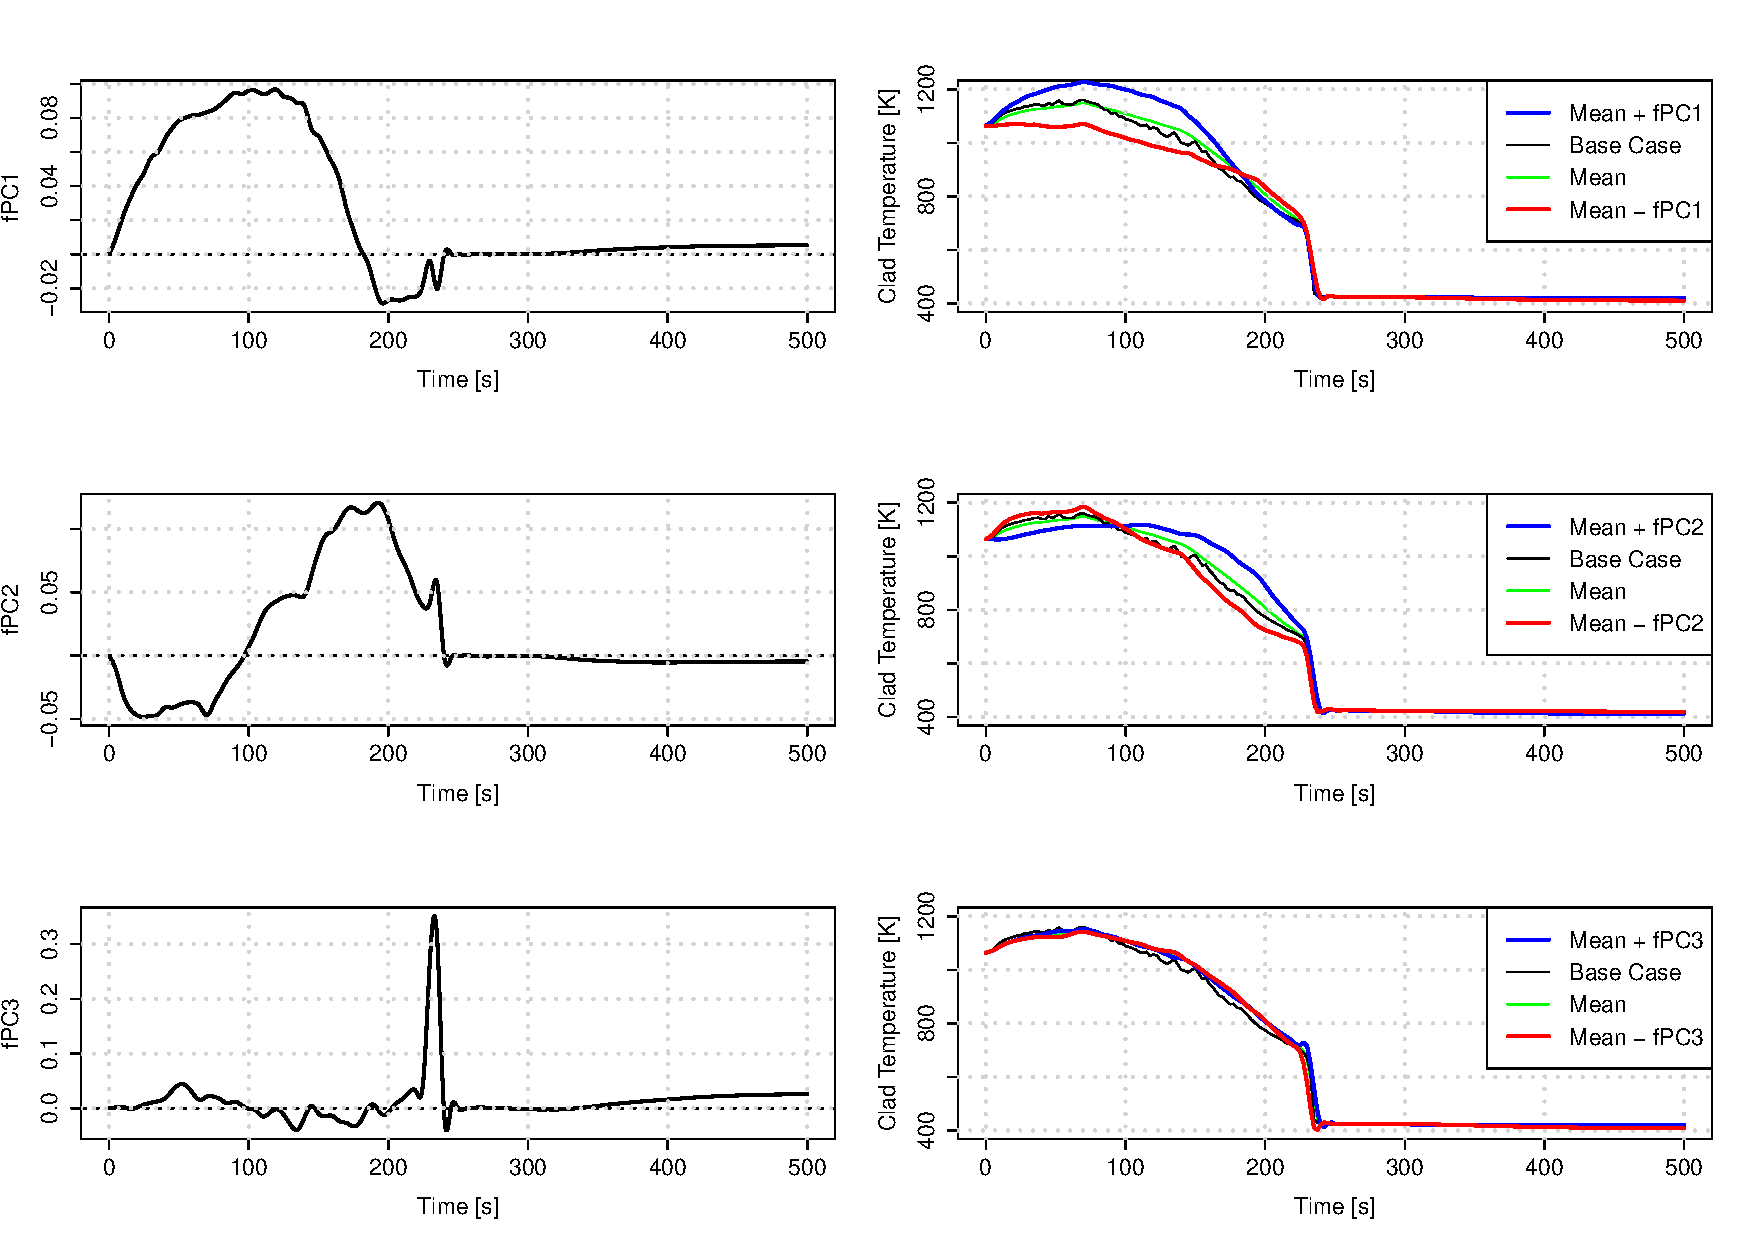
\includegraphics[width=1.1\textwidth]{figures/fpc_regfd.pdf}

        \captionof{figure}{\strut Principal modes and their effects on the
                           mean function}
    \label{fig:fpc_regfd}
\end{minipage}
\end{table}

The results of these 2 activities were summarized in two separate conference 
papers submitted to the 10\textsuperscript{th} International Topical Meeting on 
Nuclear Thermal-Hydraulics, Operation, and Safety (NUTHOS-10). 
Both papers were accepted and will be presented in the middle of December 2014 
(\cite{Wicaksono2014d,Wicaksono2014e}).

\section{Current state of work}

The current state of research during the year are summarized in 
Table~\ref{tab:currentstate} shown below.

\begin{table}[!h]
\caption{Current state of research in relation to the previously submitted
         (1\textsuperscript{st} year) work plan
         }
\centering
\label{tab:currentstate}
\scalebox{0.67}{
\begin{tabularx}{\textwidth}{@{} c Y Y Y @{}} % use 'Y' for first column
% Header ----------------------------------------------------------------------
    \toprule
    \textbf{Phase}
 & \textbf{Task Description}
 & \textbf{Planned Outcome}
 & \textbf{Current State of Work} \\ \midrule
% Table Elements --------------------------------------------------------------
   \multirow{5}{*}{\textbf{1}}                                %Phase
 & Comprehensive reviews of post-CHF flow closure             %Task Description
   laws in TRACE and externalization of important
   model parameters
 & 1 Technical Report (PSI)                                   %Planned Outcome
 & 1. Important reflood model parameters externalized         %Current State
   2. PSI contribution to OECD/NEA PREMIUM Benchmark finalized  \\ \midrule
%
   \multirow{8}{*}{\textbf{2}}                                %Phase
 & Global sensitivity analysis of important                   %Task Description
   based on FEBA test facility
 & 1 Technical Report (PSI) \& 1 Journal Article              %Planned Outcome
 & 1. A paper on Morris screening method for NUTHOS-10        %Current State
   2. Another paper on an application of functional data
      analysis for NUTHOS-10
   3. One abstract on global sensitivity analysis
      method submitted to NURETH-16      \\ \midrule
%
   \multirow{5}{*}{\textbf{3}}                                %Phase
 & Definition of error and specification of                   %Task Description
   probabilistic error model; Calibration of TRACE 
   reflood model based on the FEBA facility;
   Approximation of the posterior distribution by 
   Markov-Chain Monte Carlo; 
 & 1 Technical Report (PSI) \& 1 Journal Article              %Planned Outcome
 & $-$ \\ \midrule                                            %Current State
%
   \multirow{6}{*}{\textbf{4}}                                %Phase
 & Calibration of TRACE reflood model based on another        %Task Description
   reflood test facility
 & 1 Conference Paper                                         %Planned Outcome
 & Possible candidates of reflood facility with adequate      %Current State
   specification and
   experimental data are available (\textit{e.g.,}
   SEFLEX, NEPTUN, ACHILLES) \\ \midrule
%
   \multirow{4}{*}{\textbf{5}}                                %Phase
 & Consolidation of the calibration results based on 2        %Task Description
   facilities and validation based on another reflood
   test facility
 & 1 Journal Article                                          %Planned Outcome
 & $-$  \\\midrule                                            %Current State
%
   \textbf{6}                                                 %Phase
 & Thesis write-up                                            %Task Description
 & Thesis                                                     %Planned Outcome
 & $-$ \\                                                     %Current State
 \bottomrule
\end{tabularx}
}
\end{table}

The work in the application of global sensitivity analysis using
FDA-derived metrics as the quantities of interest is currently in-progress.
The Sobol method for variance decomposition is a step forward in extending 
the global sensitivity analysis where parameter importance are ranked by the 
nature of their interactions.
Combining these developments, further insight into the behavior and performance 
of the reflood model in TRACE can be gained especially in terms parameters 
interaction.
The interpretation of these aspects of the model are important to avoid 
ill-posedness in a parameter estimation problem.

Following a better understanding of model behavior and model parameter 
interactions through global SA, the work will continue on defining an
appropriate probabilistic error model as well as the likelihood function for
a reflood model.
This model and the function should be derived on the basis of 
probability theory and, at the same time, should also be consistent with 
the underlying models describing the reflood phenomena.

\section{Calendar of upcoming work}


\begin{table}[!h]
\caption{Calendar of upcoming work (year 2015)}
\centering
\label{tab:calendar}
\scalebox{0.79}{
\begin{tabularx}{\textwidth}{@{} c Y Y @{}} % use 'Y' for first column
% Header ----------------------------------------------------------------------
   \toprule
   \textbf{Time Frame}
 & \textbf{Task Description}
 & \textbf{Publication Outcome}\\ \midrule
% Table Elements --------------------------------------------------------------
   \multirow{5}{*}{Mid. Jan. - Mid. March}                    %Phase
 & Application of Sobol Method for reflood simulation on 
   FEBA SETF; Development of nodalization tool to fastened
   model development; Coursework
 & NURETH-16 Conference contribution\\\midrule                %Planned 
 % Table Elements -------------------------------------------------------------
   \multirow{6}{*}{Feb. - Apr.}                               %Phase
 & Comprehensive review on TRACE reflood closure laws 
   including the functions call stack structure from 
   inside the source code; Development of nodalization 
   tool to fastened model development; Coursework
 & 1 Technical report (PSI)\\\midrule                         %Planned Outcome
% Table Elements --------------------------------------------------------------
   \multirow{8}{*}{Apr. - Mid. Jun.}
 & Consolidated studies of the model review,                  %Phase
   global sensitivity analysis results (Morris and Sobol) 
   using FDA-derived quantities of interest;
   Preparation of a master thesis proposal on FDA-based 
   GSA and UQ 
   for the Achilles reflood facility; Coursework
 & 1 Journal publication (an extension of the contribution    %Planned Outcome
   to NURETH-16) \& a Master Thesis Proposal \\\midrule
% Table Elements --------------------------------------------------------------
   \multirow{5}{*}{Jul. - Mid. Aug}                           %Phase
 & TRACE assessment on the basis of FEBA 
   complemented with development of an appropriate error 
   model for functional (transient) output; Coursework
 & 1 Technical report (PSI)\\\midrule                         %Planned Outcome
% Table Elements --------------------------------------------------------------
   \multirow{5}{*}{Mid. Aug. - Sep.}                          %Phase
 & ACHILLES TRACE modeling and assessment; 
   Participate in NURETH-16 conference; Preparation
   for the master student's semester work 
   (\textit{if applicable})  
 & 1 Technical report (PSI)\\\midrule                         %Planned Outcome
% Table Elements --------------------------------------------------------------
   \multirow{6}{*}{Oct. - Dec.}                               %Phase
 & Development of probabilistic error model and simple 
   proof-of-principle on the application of Bayesian 
   updating for reflood model in TRACE; Supervision of 
   student's semester work (\textit{if applicable})
 & 1 Technical report (PSI) \& 1 Conference publication\\     %Planned Outcome
 \bottomrule
\end{tabularx}
}
\end{table}

\section{Other activities and remarks}

\subsection{NES PhD Student Day}

A poster was prepared and presented at the annual PhD Student Day of the 
Nuclear Energy Safety (NES) Department, Paul Scherrer Institut and co-sponsored 
by the \textit{Nuklearforum Schweiz}.
The poster \cite{Wicaksono2014b} was presented along with 11 other PhD students 
within NES Department to general audience.
The presentation was well-received and was selected as the best 
poster by a panel of jury.


\subsection{Nuclear Computation Lab (ETH-531)}

A teaching activity during the year 2014 was carried out for a part of  
the Nuclear Computation Lab. course given at PSI (one chapter out of six).
The course was part of the block courses offered to the EPFL/ETHZ Nuclear
Engineering Master Program.
A single day was dedicated for lecture session followed by a hands-on 
computer simulation sessions.
12 students participated in the course this semester.

In preparation for the course, the available lecture slides was fully revised
for a better structure and added with more clarifying examples.
Part of the lab. manual has also been updated for this period.
Finally, the simulation session was slightly extended with more freedom 
given to the students to set up their own model.
Helped by students' enthusiasm and interactions, the overall experience was 
positive.

\section{Scientific publications, conference contributions, and presentations}

\nocite{Wicaksono2014a}
\nocite{Wicaksono2014b}
\nocite{Wicaksono2014c}
\nocite{Wicaksono2014d}
\nocite{Wicaksono2014e}
\printbibliography[heading=none]

% Signature Page
\newpage
%\textcolor{white}.\\\\
\noindent\textbf{Comments by the thesis advisor(s)}\\\\
\noindent\textbf{Prof. A Pautz}\\\\
............................................................................
............................................................................\\\
............................................................................
............................................................................\\\
............................................................................
............................................................................\\\
............................................................................
............................................................................\\\
............................................................................
............................................................................\\\
............................................................................
............................................................................\\\
............................................................................
............................................................................\\\
............................................................................
............................................................................\\\
............................................................................
............................................................................\\\

\noindent\textbf{O. Zerkak}\\\\
\noindent Damar can be credited with a prolific and promising first phase of his research 
project. 
Despite unavoidable initial difficulties, Damar could assimilate the 
topic and rapidly become independent.
He proposed a solution approach of his own, that he will need to implement and 
test for the reflood problem next year.
His approach of combining FDA with a solution method for Bayesian inference 
problem (such as Markov Chain Monte Carlo sampling) is very original in 
the nuclear engineering field.
I should also add that Damar has proved very reliable in executing PSI 
contribution to the OECD/NEA PREMIUM project.

\section*{\underline{Signatures}\\}
\noindent \textbf{Thesis advisor}\hspace{6.25cm}\dotfill\vspace{0.5cm}\\

\noindent \textbf{Thesis co-advisor}\hspace{5.7cm}\dotfill\\
\noindent  (if officially nominated)\\\\

\noindent \textbf{With his signature, the candidate confirms that he took note 
                  of the above comments.}\\\\

\noindent \textbf{Candidate}\hspace{7cm}\dotfill\vspace{0.5cm}\\

\noindent \textbf{Date}\hspace{8.05cm}\dotfill\\

\vspace{0.8cm}
%\begin{center}
%\textbf{Up to 5 pages in total}
%\end{center}
\begin{center}
\textbf{To be returned to:} \textcolor{green}{EPFL-EDPY / Station 3 
                                              / 1015 Lausanne / Suisse}
\end{center}

\end{document}
